\chapter{Abstract}\label{cap:intro}


\begin{figure}[tbp]
\begin{center}
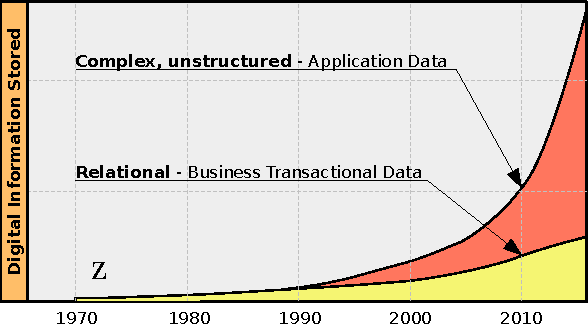
\includegraphics[width=0.6\textwidth]{imagenes/001.pdf}
 \caption{Demand in exponential growth. Source: \emph{Cloudera Inc.}}
\label{fig:datagraph}
\end{center}
\end{figure}


\noindent Over the last years there has been a continuous increase in the amount of information generated with the Internet as the main driver. Furthermore, this information has reshaped from structured --- and thus, susceptible to being expressed following a relational schema --- to heterogeneous, which has kick-started the necessity to alter the way it is stored and transformed. As the figure \ref{fig:datagraph} shows, those that were the undisputed back-end queens --- mostly relational database systems --- are seeing how their role is fading away due to their incapability to efficiently save unrelated heterogeneity.

As another related dimension, in the year 2000 many \emph{.com} companies started upgrading their data centers to accommodate the inexorable demand peak that was going to follow. But it never came; and the bubble burst. What happened then was a general underutilization --- only \texttt{10\%} of Amazon's global computational resources were in use --- that pushed the search for alternative means to export the surplus as a product. Amazon's own initiative unfolded in 2006 with the \emph{AWS} (\emph{Amazon Web Services}) appearance. AWS, among others, implements a public API for flexible on-demand infrastructure provisioning.

Since then, similar projects have proliferated generalizing how private clusters' unused computational capacity is to be serviced, trying to stay API-compatible with the AWS to facilitate interoperability and thus avoid their users' swapping to more flexible providers.

Meanwhile, Google was also in the search for new mechanisms to exploit, with high performance and securely, their own private infrastructure to evolve the capability of their services. MapReduce, as a way to massively execute thousands transformations on input data, became a reality to thrust the generation of Google's humongous inverted index of the Internet \cite{googlemapreduce}. Forthcoming contributions from Nutch's developers --- by that time an Internet search engine prototype --- to the MapReduce paradigm at \emph{Yahoo!}, would traduce into the appearance of today's \emph{de facto} standard in the field: Hadoop. Nowadays Hadoop is used in a myriad of backgrounds, ranging from travel booking sites to storing and servicing mobile data, ecommerce, image processing applications, searching for new forms of energy, business intelligence or web analytics.

So, by stacking a MapReduce implementation atop elastic infrastructure, an optimal exploitation of computational resources would be attainable rapidly expanding or shrinking them on-demand, while simultaneously reducing the overall energy consumption required to accomplish processing (Figure \ref{fig:energysavings}).

\begin{figure}[tbp]
\begin{center}
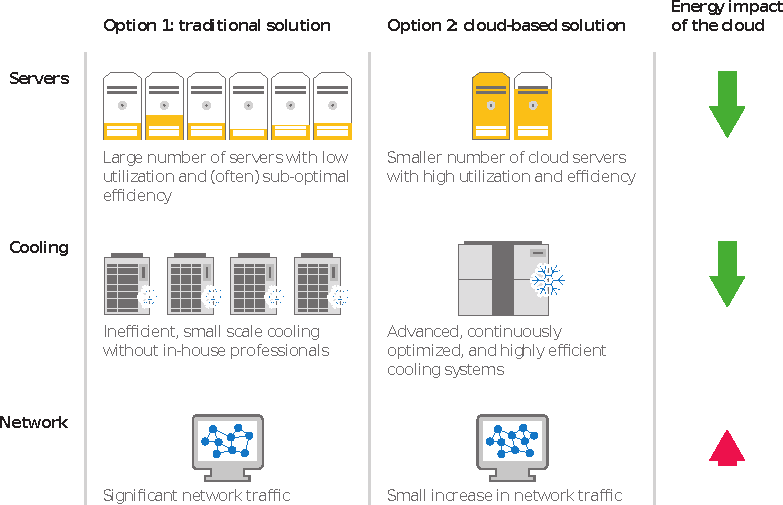
\includegraphics[width=0.9\textwidth]{imagenes/002.pdf}
 \caption{Energy savings. Source: \cite{googleapps}}
\label{fig:energysavings}
\end{center}
\end{figure}

\section{Goals}\label{sec:objetivos}
\noindent The main goal this text pursues is to study the feasibility to develop a solution for a cloud to drive MapReduce applications, with no need to know the particular cloud structure and/or Hadoop configuration parameters.

In order to achieve such a simple execution model without compromising performance or applicability, a thorough analysis of different \emph{IaaS Frameworks} will be carried out. Their features will be evaluated inside a virtual testing environment to finally narrow the selection to only one. Once an IaaS Framework had been chosen, the attention will be put towards choosing a MapReduce implementation to install over our virtual infrastructure.

Nonetheless, a mechanism to forward MapReduce execution requests will be devised and implemented trying to focus on simplicity and universal access to this human-cloud-mapreduce interface. Yet, this transparency mustn't become an obstacle in exploiting the application or in fetching processed results. Privacy and security in communications and storage will be conveniently defined; we shan't forget it will be developed as a scaled-down model which could be infinitely scaled out.

\section{Arrangement of the Document}\label{sec:organizacion}
\noindent The contents within this document are distributed as stated next. This first chapter introduces development guidelines in the abstract. Chapter \ref{cap:estadodelarte} puts the reader closer to the fundamental Cloud Computing concepts --- like general architecture or virtualization ---, along with those from the MapReduce paradigm. Chapter \ref{cap:evaliaas} describes an empirical evaluation of four private IaaS Cloud frameworks. Chapter \ref{cap:openstack} explores OpenStack Folsom's modular structure and particular inner workings. Likewise, chapter \ref{cap:hadoop} unveils Hadoop's peculiarities as a MapReduce implementation.

The subsequent chapters center on detailing the project from diverse vantage points. Chapter \ref{cap:solucion} contains a series of design decisions and their accompanying UML diagrams. Chapter \ref{cap:rendimiento} gathers an analysis on performance in a real testing cluster. Chapter {cap:conclusiones} analyzes related papers highlighting how they compare to this solution. Finally, the main contributions of this project are discussed in addition to proposing future improvements to the implementation.

Two annexes have also been included. Annex \ref{cap:guiainstalacion} guides the reader throughout a quick single node installation and its operating maintenance. Annex \ref{cap:glosario} covers the definition of some of the concepts and technologies referred to in this text.
